\documentclass[twocolumn,prd,nofootinbib]{revtex4}
%\newcommand\ForRichardOnly[1]{#1}
\newcommand\ForRichardOnly[1]{}
\usepackage{verbatim}
\usepackage{color}     % color text
\usepackage{framed}
\definecolor{shadecolor}{gray}{0.95}
\usepackage{amsmath}
\usepackage{graphicx}  % extend graphics
\usepackage{tabularx}
\usepackage{wrapfig}   % wrap text around figures, if desired
\usepackage{hyperref}

\newcommand\ForInternalReference[1]{#1}
%\newcommand\ForInternalReference[1]{}

\newcommand\Y[1]{Y^{(#1)}{}}
% GR tools
\newcommand\prederiv[2]{{}^{(#1)}#2}
\newcommand\dualBack{*}
\newcommand\dualForward{\star}
\newcommand\avL{\left< {\cal L}_{(a} {\cal L}_{b)} \right>}
\newcommand\WeylScalar{{\psi_4}}
\newcommand\WeylScalarFourier{{\tilde{\psi}_4}}
\newcommand\mc{{{\cal M}_c}}
% QM TOOLS
\newcommand\qmstate[1]{\left|#1\right \rangle}
\newcommand\qmstateKet[1]{\left\langle#1\right|}
\newcommand\qmstateproduct[2]{\left\langle#1|#2\right\rangle}
\newcommand\qmoperatorelement[3]{\left\langle#1\left|#2\right|#3\right\rangle}
\newcommand\qmoperator[1]{{\bf #1}}


\begin{document}

\title{Rapid, embarassingly parallel parameter estimation of gravitational waves from compact binary coalescences}
\author{P. Brady}
\email{patrick@gravity.phys.uwm.edu}
\affiliation{Center for Gravitation and Cosmology, University of Wisconsin-Milwaukee, Milwaukee, WI 53201, USA }
\author{E. Ochsner}
\email{evano@gravity.phys.uwm.edu}
\affiliation{Center for Gravitation and Cosmology, University of Wisconsin-Milwaukee, Milwaukee, WI 53201, USA }
\author{R. O'Shaughnessy}
\email{oshaughn@gravity.phys.uwm.edu}
\affiliation{Center for Gravitation and Cosmology, University of Wisconsin-Milwaukee, Milwaukee, WI 53201, USA }
\author{C. Pankow}
\email{pankow@gravity.phys.uwm.edu}
\affiliation{Center for Gravitation and Cosmology, University of Wisconsin-Milwaukee, Milwaukee, WI 53201, USA }

\begin{abstract}
We present a method for rapid, parallelizable parameter estimation  of GWs from CBCs.
\end{abstract}
\maketitle

\begin{widetext}
\section*{Outline}
The first level of bullets are proposed sections. 
The second level of bullets (except in Executive Summary) are proposed subsections.
The third level of bullets are points to make in each subsection.

Section headings added, including reminders re dotting i's/crossing t's.

\begin{itemize}
\item Executive Summary
	\begin{itemize}
	\item Goal: Rapid parameter estimation of CBC GW signals -- target is a few minutes!
	\item Trick \# 1: use mode decomposition and compute $( h_{\ell m} | d )$ once for each mass pair.
		Extremely fast likelihood evaluation as extrinsic parameters are varied.
	\item Trick \# 2: Abandon Markov chain/ nested sampling. They have nice convergence in high dimensions,
		but are serial. Instead, use brute force grid and Monte Carlo technique. Convergence worse in a sense,
		but embarassingly parallel and very rapid evaluations thanks to trick \# 1.
	\item Essentially same cost regardless of waveform evaluation speed. Therefore can use very long signals 
		and/or expensive models like EOB. 
	\end{itemize}

\item Methods
	\begin{itemize}
        \item Background
           
	\item Likelihood evaluation
		\begin{itemize}
		\item Start with expression for ${\cal L}$. 
		\item Show steps to get in terms of $( h_{\ell m} | d )$.
		\item Note how all extrinsic parameters enter in $Y_{\ell m}$'s and $F_+$, $F_\times$, and thus we can
			evaluate likelihood cheaply for any extrinsic parameters if we fix the intrinsic ones.
		\end{itemize}
		
		
	\item Integration over extrinsic parameters
		\begin{itemize}
		\item Do a basic Monte Carlo integral over  extrinsic parameters, at fixed intrinsic parameters
                        Priors (e.g., time window)
%		\item Describe any fancy pants adaption, use of skymaps, etc. 
		\end{itemize}
                \begin{itemize}
  	         \item Time marginalization  \textbf{subsection of extrinsic} 
		  \begin{itemize}
		  \item Inverse FFT trick gives $(h_{\ell m}(t_c) | d)$ for all values of $t_c$ at once.
		  \item We just sum over a reasonably sized window $\sim 10$ ms. 
		  \end{itemize}
                 \item Adaptation (in distance)
                 \item Targeted sampling : skymaps
                \end{itemize}

	\item Covering the intrinsic parameters
		\begin{itemize}
		\item Describe effective Fisher approach to laying out mass points.
		\item Point out quite flexible: can do random or fixed grid, can change ellipse size, distribution inside ellipse,
			could do several ellipses centered on different points. [?]
		\item Point out difficult to go to many intrinsic dimensions. Right now we focus on 2D non-spinning, 
			but 3D or 4D is possibly feasible.
			Precession would be very tough. 
			Maybe an approximate metric or help from ROM could save the day. [?]
		\end{itemize}
		
	\end{itemize}
	
	\item Postprocessing [?]
		\begin{itemize}
		\item Do we need to say anything about collating results, making triplots, P-P plots, etc.?
		\end{itemize}

\item Results
	\begin{itemize}
	\item Show posteriors, convince reader they're similar enough to usual Bayesian PE to be trusted.
	\item P-P plots. Show our results are self-consistent.
	\item Brief (not more than 1-2 paragraphs, 1 simple plot/table) results confirming 
		that our method scales favorably with $f_{\rm min}$ and/or EOB. 
	\end{itemize}

\item Conclusions -- self-explanatory.

\item Appendices -- Put detailed technical asides here.

\end{itemize}

Citations: Bayesian methods and monte carlo integration \cite{2011RvMP...83..943V}, including numerical recipes and Lepage; comparison
to other PE methods for LIGO
(MCMC,nested sampling) \cite{LIGO-CBC-S6-PE,2011PhRvD..83h2002D,2011PhRvD..84f2003C,gr-extensions-tests-Europeans2011,gwastro-mergers-PE-Aylott-LIGOATest,2011ApJ...739...99N,2012PhRvD..85j4045V,gw-astro-PE-Raymond,gw-astro-PE-lalinference-v1}

\tableofcontents

\end{widetext}

\section{Introduction}

\section{Executive Summary}

Here's the executive summary.

\section{Methods}

Methods go here.

\subsection{Efficiently evaluating the likelihood}

* coordinates [limit to nonprecessing?]

\subsection{Sampling the extrinsic parameters}

\subsection{Scalable method to explore intrinsic parameters }


\section{Results}

Results go here.

\subsection{Scaling}

\subsection{Detailed investigation of one event}

Sample run results: extrinsic parameters (for one and several noise realizations)

Sample run results: $L_{\rm red}(\mc,eta)$ (for one and several noise realizations). Expected accuracy at each mass
point.. Translating into  $p(m_1,m_2)$ using a uniform mass prior.

Comparison with Fisher and MCMC



%%
%% WHAT FIGURES SHOULD BE : zero noise MDC, at injected values
%%
%% WHAT FIGURES CURRENTLY ARE : https://ldas-jobs.ligo-wa.caltech.edu/~oshaughn/BNS_2015_MDC/coinc_id_10202/ or 12635
%%   (=a real result from our large-scale run MDC, adapting on the sky and distance)
%%
%% For comparison, off-master results with no adaptation in sky, diffusion, and tempering: https://ldas-jobs.ligo.caltech.edu/~oshaughn/BNS_2015_MDC/coinc_id_10202/
\begin{figure*}
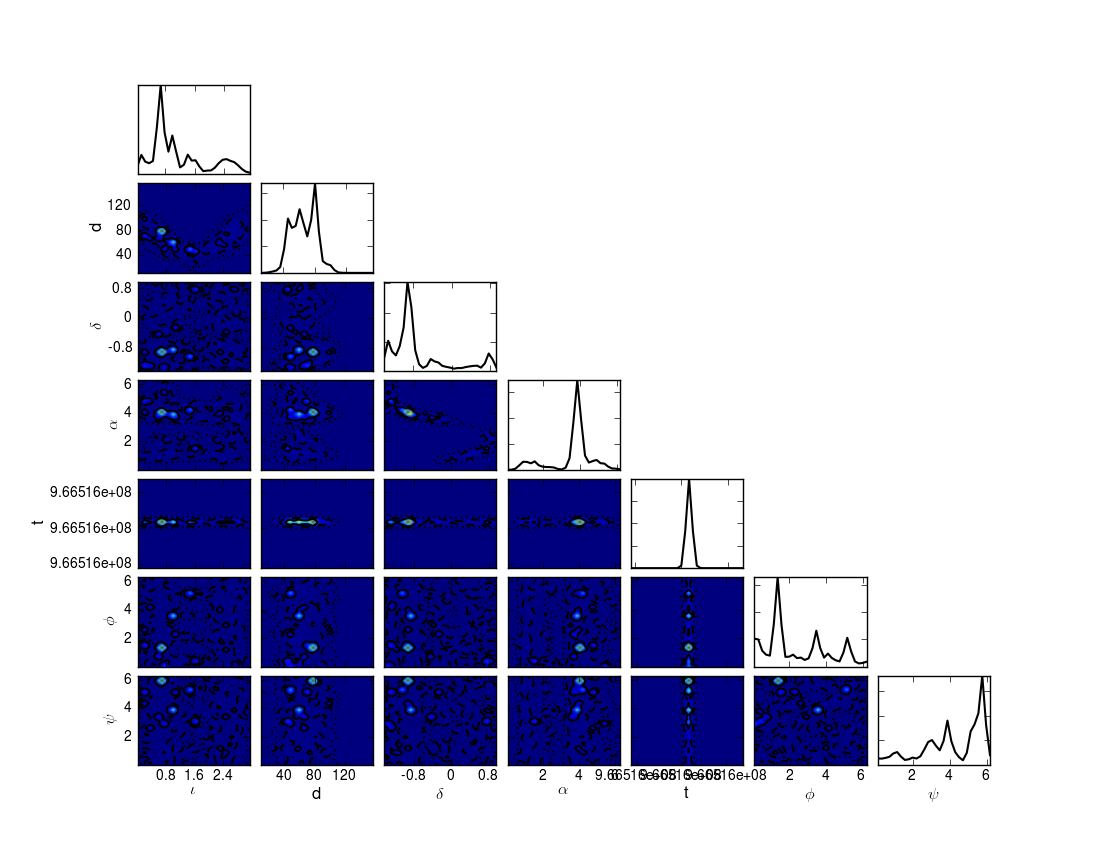
\includegraphics[width=\textwidth]{../Figures/ILE_MASS_SET_0-triplot}
\caption{\textbf{Posterior distribution in intrinsic parameters, assuming known masses}: For our fiducial event, our predicted
  distribution of extrinsic parameters $d,RA=\alpha,DEC=\delta,\iota,t,\phi,\psi$, assuming the exact parameters are
  known.    \textbf{PLACEHOLDER} \emph{Suggest: show d-cos iota, skymap, and phi-psi only, not full triplot}
}
\end{figure*}


\begin{figure}
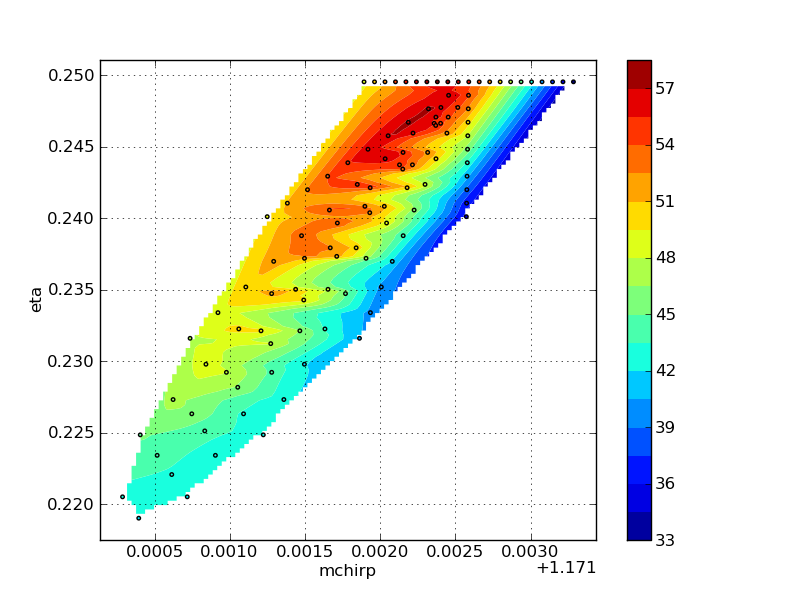
\includegraphics[width=\columnwidth]{../Figures/coinc_id_12635_mchirp_eta_logevidence}
\caption{\textbf{Marginalized likelihood and posterior distribution versus component masses}: \emph{Top panel}: For our fiducial event,
  contours of the log of integrated likelihood $\ln L_{\rm red}$ versus component masses, represented in $\mc,\eta$
  coordinates.  Points indicate the mass grid adopted; colors and the color bar indicate specific numerical values.   
\emph{Bottom panel}: The 90\% confidence interval derived from $L_{\rm red}$, for several noise realizations.  For
comparison, the prediction from a Fisher matrix is shown as a solid black curve.
 \textbf{PLACEHOLDER/INTENT}
}
\end{figure}


\subsection{Ensemble of events}

pp plots

\begin{figure}
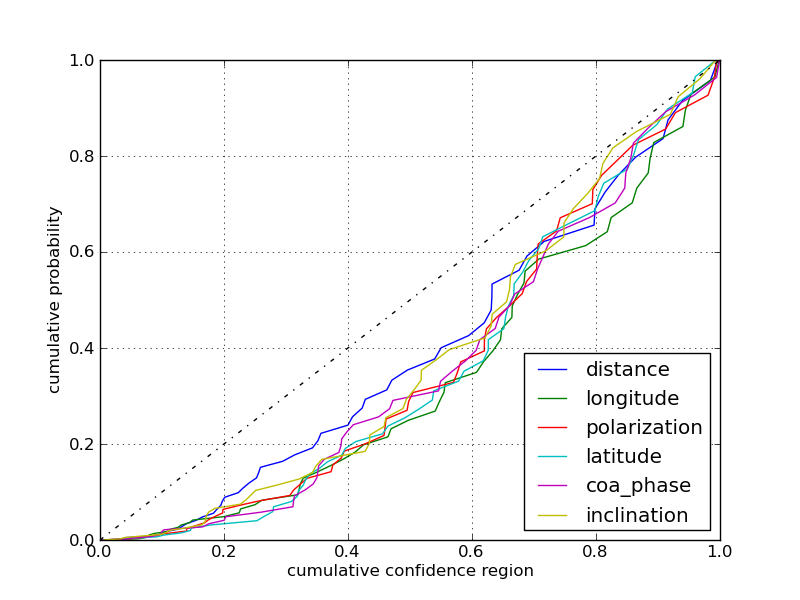
\includegraphics[width=\columnwidth]{../Figures/BNS_2015_MDC_test_pp_plot}
\caption{\textbf{PP plot for ensemble of XXX NS-NS events}: For \textbf{X} randomly-selected NS-NS binaries, a plot of
  the cumulative distribution of $P_\theta(\theta_k)$ for each extrinsic variable $\theta=d,RA,DEC,\iota,\psi,\phi_{\rm orb}$.
}
\end{figure}


\section{Conclusions}

Conclusions go here.

\appendix


\section{Notation, definitions, and equations}

\subsection{Definitions}
\begin{itemize}
\item $\lambda$ : intrinsic coordinate, including masses and spins.

\item $\theta$ : extrinsic coordinate, including $d,RA,DEC,\iota,\psi_L,t,\phi_{\rm orb}$

\item $p_s(\theta)$: (joint) sampling prior in extrinsic dimensions

\item $p(\theta)$ : prior on extrinsic parameters

\item $L(\lambda,\theta)$ : likelihood.  In terms of individual detector strains $H_k$ and power spectra, provided by
\begin{eqnarray}
\ln L &\equiv \sum_k \ln L_k  = \ln L_{\rm model} + \ln L_{\rm data} \\
\ln L_{\rm model} &\equiv -\frac{1}{2} \sum_k \qmstateproduct{H_k}{H_k}_k  \\
\ln L_{\rm data} &\equiv  \sum_k \text{Re} \qmstateproduct{H_k}{\hat{H}_k}_k 
\end{eqnarray}

\item $Z(\lambda) \equiv L_{\rm red}(\lambda,\theta)$ : reduced or integrated likelihood, derived from $L$ via
\begin{eqnarray}
Z(\lambda) = L_{\rm red}(\lambda) = \int d\theta \; p(\theta) L(\lambda,\theta)
\end{eqnarray}

\item 
$w=Lp/p_s$ : weight

\item 
$n_{\rm eff}$ : ``effective number of samples''
\begin{eqnarray}
n_{\rm eff} \equiv  \frac{\sum_k w_k}{\text{max}_k w_k}
\end{eqnarray}

\item 
$h(t|\lambda,x)=h_+-i h_\times$ : complex gravitational wave strain

\item 
$h_{lm}(t)$: coefficients of a spin-weighted spherical harmonic decomposition
\begin{eqnarray}
\label{eq:def:hSpinWeightEmissionDirection}
h(t|\lambda,\theta) = \sum_{lm} h_{lm}(t|\lambda) e^{-2i\psi_J}\Y{-2}_{lm}(\theta_{JN}\phi_{JN})
\end{eqnarray}

\item 
$\tilde{h}(f)$ : two-sided Fourier transform of the complex function $h(t)$
\begin{eqnarray}
h(t) = \int_{-\infty}^{\infty} \frac{d \omega}{2\pi} \; e^{-i\omega t} \tilde{h}(\omega) 
\end{eqnarray}

%% \item
%% ${\cal I}$ : complex conjugation in time.  Provided to avoid confusion with $\tilde{h}^*$.  \textbf{Hopefully we won't
%%   need it.}


\item 
$\vec{x}_k$ : Position of the $k$th detector

\item 
$F_{+}$, $F_{\times},F$ : detector response function  to the $+,\times$ polarizations for sources visible in the
  $\hat{n}$ direction from the detector
\begin{eqnarray}
F(\hat{n}) = F_+(\hat{n}) +i F_\times(\hat{n})
\end{eqnarray}

\item 
$H_k$ : strain response of the $k$th detector to an incident strain
\begin{align}
H_k(t) &=F_{+,k}(t) h_+(t-\vec{x}_k(t)\cdot \hat{k}) + F_\times(t) h_\times(t-\vec{x}_k(t)\cdot \hat{k}) \\
 &=  \frac{F h(t-\vec{x}_k\cdot \hat{k}) }{2} + \frac{F^*h^*(t-\vec{x}_k\cdot \hat{k})}{2}
\end{align}

\item 
$S_k$ : noise power spectrum for the $k$th detector

\item 
$\qmstateproduct{a}{b}_k$ : complex-valued inner product defined by the $k$th detector's noise power spectrum:
\begin{eqnarray}
\qmstateproduct{a}{b}_k \equiv 2 \int_{-\infty}^{\infty} df \frac{[\tilde{a}(f)]^*\tilde{b}(f)}{S_h(|f|) }
\end{eqnarray}


\item 
$Q_{k,lm}(\tau)$ : complex-valued single-detector, single-harmonic ``SNR'' series
\begin{eqnarray}
Q_{k,lm}(\tau) \equiv \qmstateproduct{\exp(-i\omega \tau) h_{lm}}{\hat{H}_k}_k
\end{eqnarray}

\end{itemize}

\subsection{Other assumptions}
Assuming the earth does not rotate significantly during the signal, allowing us to approximate
\begin{eqnarray}
\qmstate{H_k} = \frac{e^{i\omega \hat{k}\cdot \vec{x}_k}}{2}\left[ 
   F_k  \qmstate{h} + F_k^* \qmstate{h^*} 
 \right]
\end{eqnarray}


\begin{widetext}
\subsection{Core equations}

\begin{align}
\ln L_{\rm data}(\lambda|t,\hat{n},\hat{k},\psi_J,d) &=  \sum_k\qmstateproduct{H_k}{\hat{H}_k}_k \nonumber \\
\label{eq:Implementation:lnLData}
&= (d_{\rm ref}/d) \text{Re} \sum_k \sum_{lm}(F_k(-\hat{k}) e^{-2\psi_J} \Y{-2}_{lm}(\hat{n}))^* Q_{k,lm}(t-\hat{k}\cdot x_k)
\end{align}

\begin{subequations}
\label{eq:ComputeRhoViaInnerProductMatrix}
\begin{align}
{ U_{k,lm,l'm'}(\lambda)}& = \qmstateproduct{h_{lm}}{h_{l'm'}}_k \\
V_{k,lm,l'm'}(\lambda)& = \qmstateproduct{h_{lm}^*}{h_{l'm'}}_k \\
\ln L_{\rm model}(\lambda|\hat{n},\hat{k},\psi_J,d) &=
   -\frac{(d_{\rm ref}/d)^2}{2}\sum_k
\left[
{
 \frac{1}{2}|F_k(-\hat{k})|^2 U_{k,lm,lm'}(\lambda)[\Y{-2}_{lm}(\hat{n})]^*\Y{-2}_{l'm'}(\hat{n})
}
 \right. \nonumber \\ & \left.
 {
+
 \frac{1}{2} \text{Re} V_{k,lm,l'm'} e^{-4i\psi_J}F_k^2 \Y{-2}_{lm}(\hat{n})\Y{-2}_{l'm'}(\hat{n})
}
\right]
\end{align}
\end{subequations}


One-dimensional marginalized posteriors, generally and sampled: 
\begin{eqnarray}
p_1(x_1|{\cal D}) dx_1 \equiv \int p(x|{\cal D} dx = \frac{dx_1}{Z} \int dx_{2}\ldots dx_n p(x_2)\ldots p(x_n)L(x_1\ldots x_n) 
\end{eqnarray}
\begin{eqnarray}
\hat{p}_1(z) \equiv \frac{1}{N \hat{Z}}\sum_{k=1}^N K(x,x_k) \frac{L_k p_k}{p_{s,k}} 
\; ; \qquad
\hat{Z} \equiv \frac{1}{N} \sum_{k=1}^N \frac{L_k p_k}{p_{s,k}}
\end{eqnarray}
where $K(x,y)$ is some normalized ($\int K(x,y) dx = 1$) kernel  and where $\hat{Z}$ is our running
estimate for the evidence ($Z = \int L p dx$).


\end{widetext}

\ForInternalReference{
\section{[Internal use] Incomplete or not-yet-implemented investigations}

\subsection{Measures of convergence}

Measures to assess whether we're done
\begin{itemize}
\item * Integral: Classic MC error estimate (central limit); reproducibility across runs and via subsamples (e.g., chisquared)

\item * 1d posterior:  $n_{\rm eff}$; $L^2$ or KL divergence between subsamples or across runs

\item * sampling distribution: similarly
\end{itemize}


\subsection{Semianalytic marginalization over distance}


\section{[Internal use] Future directions}


}
\bibliography{overviewexport}
\end{document}
